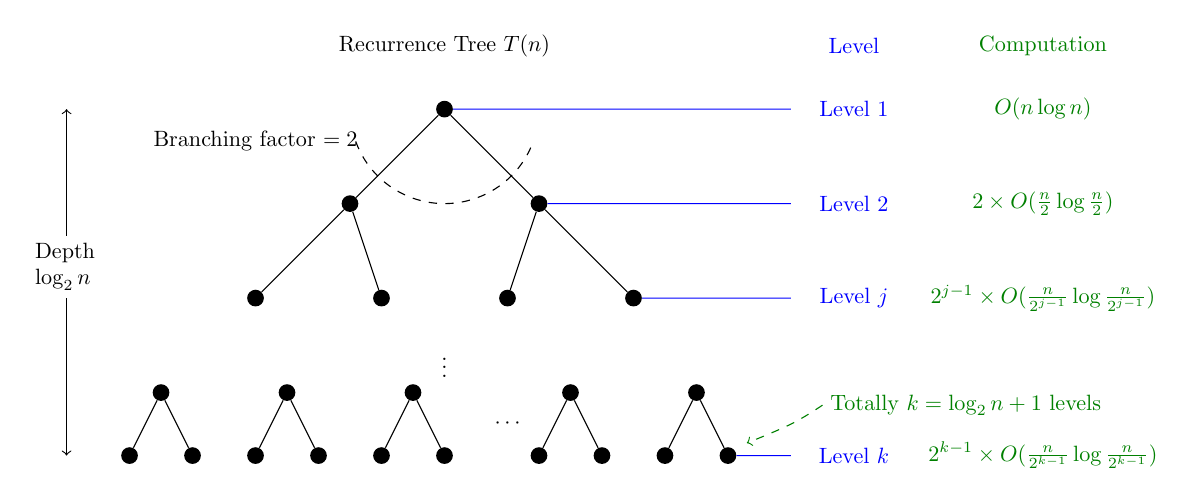
\begin{tikzpicture}[scale=0.8,every node/.style={scale=0.8}]
\tikzstyle{bdot} = [fill=black,circle,scale=0.8];
\tikzstyle{lv} = [blue];
\tikzstyle{comp} = [green!50!black];
\tikzstyle{blueline} = [blue]
\node[bdot] (v1) at (0,2.5) {};
\node[bdot] (v2) at (-1.5,1) {};
\node[bdot] (v4) at (1.5,1) {};
\draw[dashed] (-1.4095,1.987) arc (-160.0006:-20:1.5);
\node at (-3,2) {Branching factor $=2$};
\node at (0,3.5) {Recurrence Tree $T(n)$};
\draw  (v1) edge (v2);
\draw  (v1) edge (v4);
\node [bdot] (v5) at (-3,-0.5) {};
\node [bdot] (v7) at (-1,-0.5) {};
\draw  (v2) edge (v5);
\draw  (v2) edge (v7);
\node [bdot] (v8) at (1,-0.5) {};
\node [bdot] (v10) at (3,-0.5) {};
\draw  (v4) edge (v8);
\draw  (v4) edge (v10);
\node[lv] at (6.5,3.5) {Level};
\node[lv] at (6.5,2.5) {Level 1};
\node[comp] at (9.5,3.5) {Computation};
\node[comp] at (9.5,2.5) {$O(n\log n)$};
\node [lv] at (6.5,1) {Level 2};
\node [comp] at (9.5,1) {$2\times O(\frac{n}{2}\log\frac{n}{2})$};
\node [lv] at (6.5,-0.5) {Level $j$};
\node [comp] at (9.5,-0.5) {$2^{j-1}\times O(\frac{n}{2^{j-1}}\log \frac{n}{2^{j-1}})$};
\node at (0,-1.5) {$\vdots$};
\node [bdot] (v3) at (-4.5,-2) {};
\node [bdot] (v6) at (-5,-3) {};
\node [bdot] (v12) at (-4,-3) {};
\node [bdot] (v9) at (-2.5,-2) {};
\node [bdot] (v11) at (-3,-3) {};
\node [bdot] (v13) at (-2,-3) {};
\node [bdot] (v14) at (-0.5,-2) {};
\node [bdot] (v15) at (-1,-3) {};
\node [bdot] (v16) at (0,-3) {};
\node [bdot] (v17) at (2,-2) {};
\node [bdot] (v18) at (1.5,-3) {};
\node [bdot] (v19) at (2.5,-3) {};
\node [bdot] (v20) at (4,-2) {};
\node [bdot] (v21) at (3.5,-3) {};
\node [bdot] (v22) at (4.5,-3) {};
\draw  (v3) edge (v6);
\draw  (v9) edge (v11);
\draw  (v3) edge (v12);
\draw  (v9) edge (v13);
\draw  (v14) edge (v15);
\draw  (v14) edge (v16);
\draw  (v17) edge (v18);
\draw  (v17) edge (v19);
\draw  (v20) edge (v21);
\draw  (v20) edge (v22);
\node at (1,-2.5) {$\cdots$};
\node [lv] at (6.5,-3) {Level $k$};
\node [comp] at (9.5,-3) {$2^{k-1}\times O(\frac{n}{2^{k-1}}\log \frac{n}{2^{k-1}})$};
\node [comp,right] at (6,-2.2) {Totally $k=\log_2 n+1$ levels};
\draw[->,dashed,green!50!black]  plot[smooth, tension=.7] coordinates {(6,-2.2) (5.5,-2.5) (4.8,-2.8)};
\draw[<->] (-6,2.5) -- (-6,-3);
\node[fill=white,text width=1cm] at (-6,0) {Depth $\log_2 n$};
\draw [blueline](5.5,2.5) -- (v1);
\draw [blueline](v4) -- (5.5,1);
\draw [blueline](v10) -- (5.5,-0.5);

\draw [blueline](v22) -- (5.5,-3);
\end{tikzpicture}
